\documentclass{beamer}

\usepackage[utf8]{inputenc}
\usepackage[T1]{fontenc}

\title{MicMac -- a global overview}
%\subtitle{Beamer demonstration: longer subtitle}
\institute{IGN}
\date[25 May 2018]{Technical seminar}
\author[E Rupnik]{E Rupnik, J-M Muller, M Pierrot Deseilligny} 

\newcommand{\todo}[1]{\textcolor{red}{#1}}

\usetheme{ign}

\begin{document}


    \begin{frame}[plain]
        \titlepage{}
    \end{frame}

	\tableofcontents
	
%%%%%%%%%%%%%%%%%%%%%%%%%%%%%%%%%%%%%%%%%%%%%%%%%%%% Bilans de la prese
%1/ er: introduction/overview of the processing pipeline    ~3 slides ~3mins
%2/ jmm: tie points extraction
%		+no a priori, extraction algos                      ~2-3      ~3mins
%       +with a priori,                                     ~2-3      ~3mins
%		+reduction algos                                    ~2        ~2mins

%3/ er: image orientation
%       sfm				                                    ~2-3      ~3mins
%       BBA                                                 ~2-3      ~3mins
%       structureless BBA                                   ~2-3      ~3mins
%4/ er: georef                                              ~1-2      ~1mins
	
	
%%%%%%%%%%%%%%%%%%%%%%%%%%%%%%%%%%%%%%%%%%%%%%%%%%%% Introduction        
      \section{Introduction}  
        \subsection*{The processing pipeline}
            \begin{frame}{Overview of the processing pipeline}
                %\framesubtitle{The proof uses \textit{reductio ad absurdum}.}
                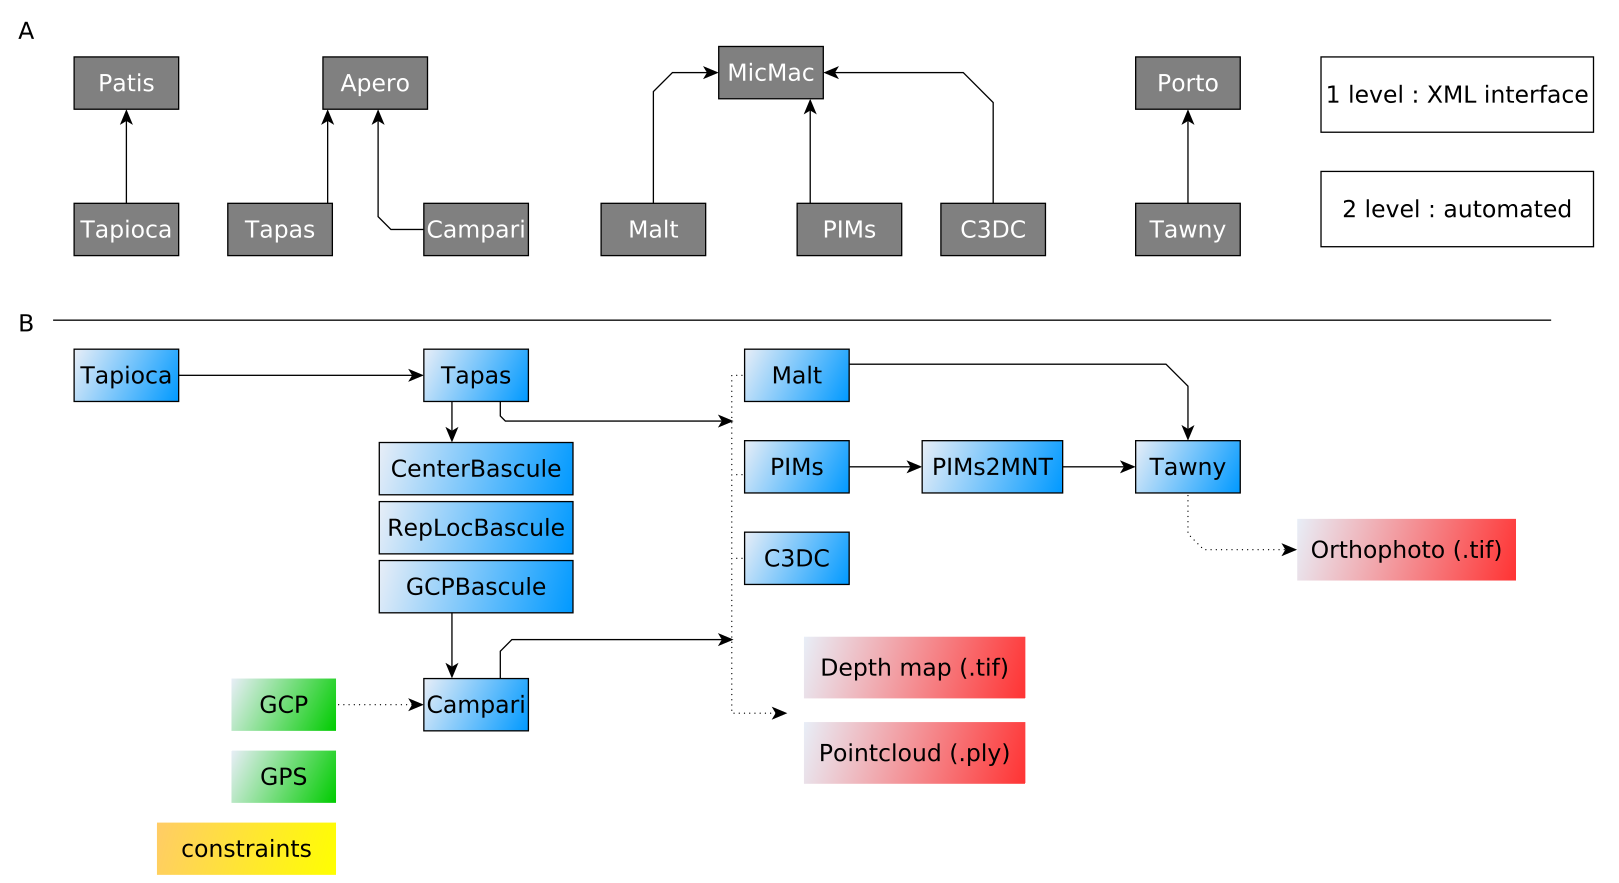
\includegraphics[width=10cm]{images/architecture_prntscr.png}
                
%change the graphic:
% remove A (and fix Patis->Pastis)
% make depth map on the right of Malt&co
% add more descriptive names (or maybe in items below Tapas=corresp)                
% introduce tool by tool on diff slides
                
            \end{frame}


%%%%%%%%%%%%%%%%%%%%%%%%%%%%%%%%%%%%%%%%%%%%%%%%%%%% Tie-points
\section{Tie points extraction}
\subsection{Without a priori geometry}
        \begin{frame}{Tie points extraction }
                \framesubtitle{Without \textit{a priori} geometry}

                \begin{block}{Tie points detection}
                        \begin{itemize}
                        \item SIFT : default
                        \item Digeo : slightly faster, possibility to use only max or min
                        \item AIME (presented by MPD during spotlight), under developpment; generally faster than SIFT
                        \end{itemize}
                \end{block}
                
                \begin{block}{Tie points Matching}
                \begin{itemize}
                        \item ANN (Approximate Nearest Neighbor)
                        \item for a point in pic A, find best and second best points in pic B.
                        The best point is accepted if his score is high and second best score is low.
                        \end{itemize}
                \end{block}
                
        \end{frame}
        
        \begin{frame}{Tie points extraction }
                \framesubtitle{Without \textit{a priori} the geometry}   
                \begin{block}{Extraction organization : lists of pictures pairs}
                \begin{itemize}
                        \item All, MulScale, Line...
                        \item from an orientation (GPS, approximate orientation)
                \end{itemize}
                \end{block}
                \textbf{Tapioca} command. See §3.3 and §16 of documentation.
                
                \begin{block}{Tie points files format (binary and ASCII)}
                \begin{itemize}
                        \item Default : 1 file per pair, simple and universal
                        \item New format : 1 file with points multiplicity, faster but only usable with few commands
                \end{itemize}
                \end{block}
                \textbf{mm3d TestLib ConvNewFH} command. See §16.8 of documentation.
        \end{frame}

\subsection{With a priori geometry}        
        \begin{frame}{Tie points extraction}
                \framesubtitle{With \textit{a priori} geometry}
                \begin{itemize}
                        \item ``Second iteration'': using camera orientations and a 3d mesh
                        \item finds tie points with good repartition on pictures and 3d mesh
                        \item use orientations for perspective corrections before correlation
                \end{itemize}
                \textbf{mm3d TiePTri} command. See §16.9 of documentation.
                
                \centering{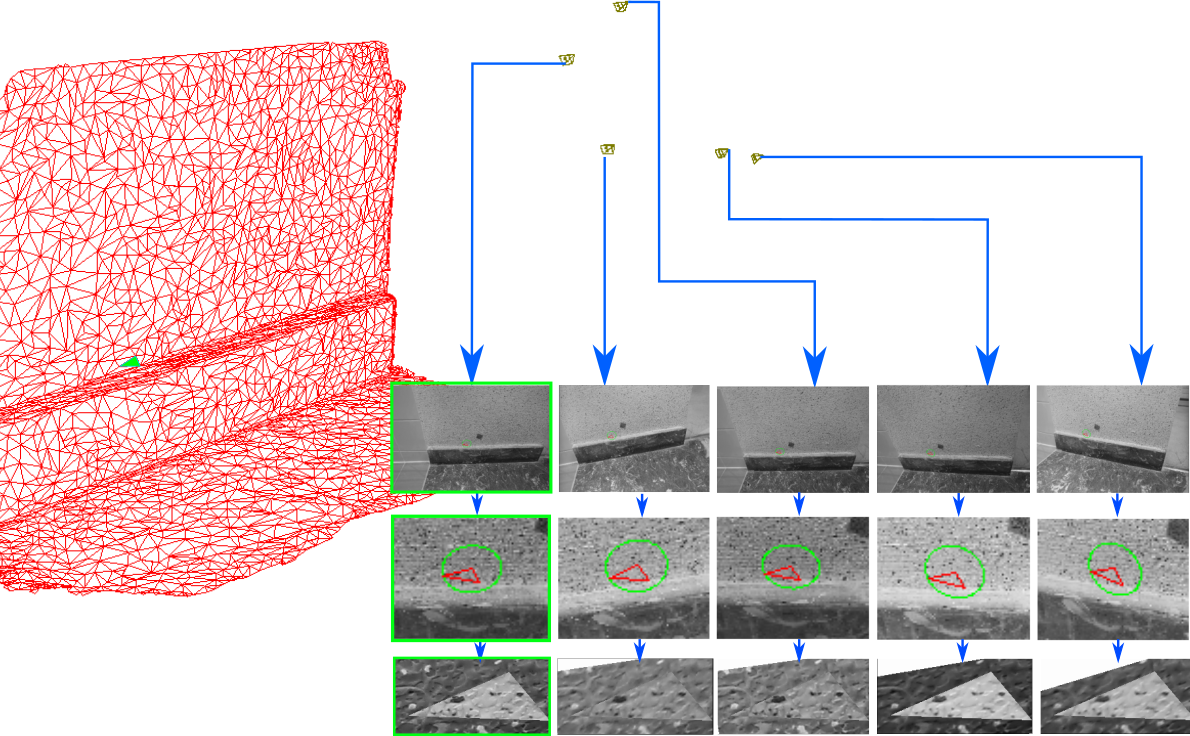
\includegraphics[width=7cm]{images/imgselect_brief}}
        \end{frame}

\subsection{Reduction algorithms}
        \begin{frame}{Tie points reduction algorithms}
                Four tools are dedicated to Tie points reduction: 
                \begin{itemize}
                        \item \textbf{RedTieP} / \textbf{Schnaps} (generic case): only one point per picutre part, favor manifold
                        \item \textbf{OriRedTieP} / \textbf{Ratafia} (quasi-vertical case) : favor scene repartition
                \end{itemize}
                
                \centering{
                        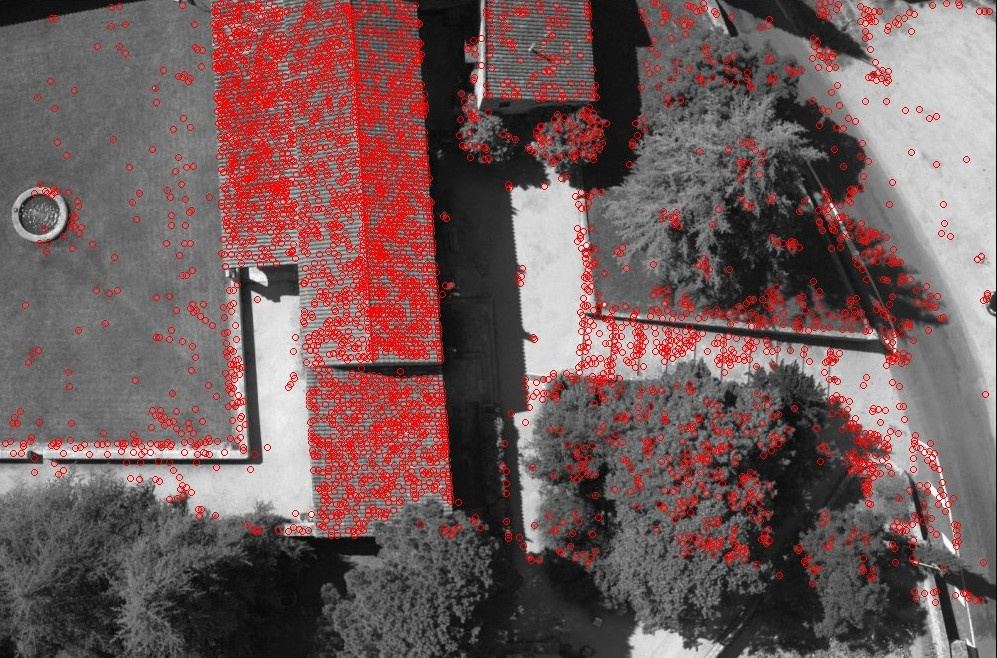
\includegraphics[width=5cm]{images/Schnaps_homol_all} \ 
                        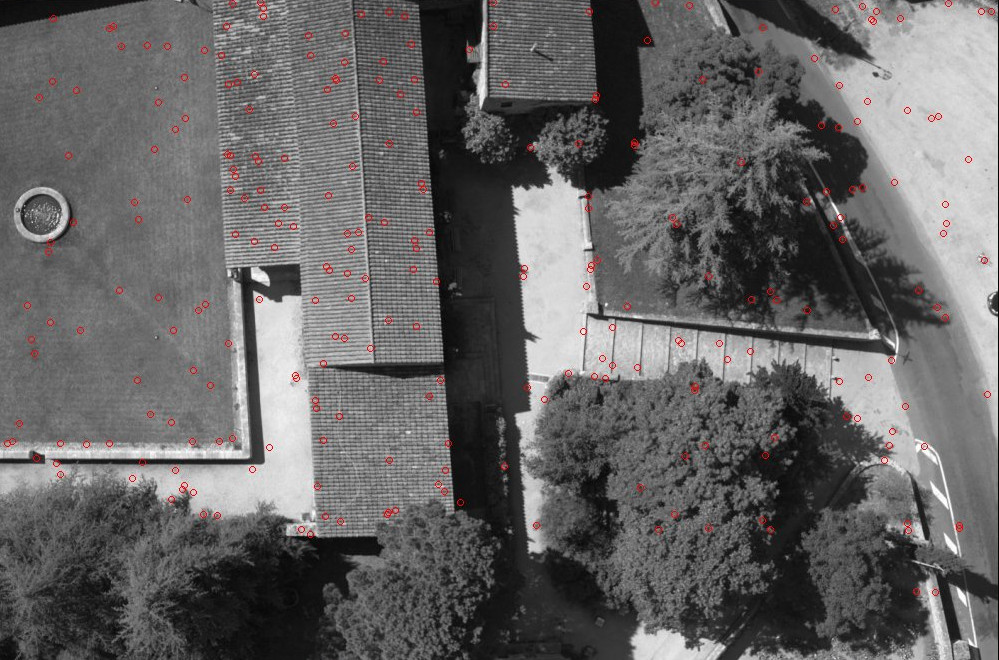
\includegraphics[width=5cm]{images/Schnaps_homol_100}
                }
                
        \end{frame} 
                        
                 
%%%%%%%%%%%%%%%%%%%%%%%%%%%%%%%%%%%%%%%%%%%%%%%%%%%% Pose estimation
\section{Image orientation}       
		\begin{frame}{Image orientation}
			\framesubtitle{Approaches}
			\begin{enumerate}
			\item no a priori, iterative (i.e. SfM)
			\item with a priori, collinearity-based bundle block adjustment (BBA) when initial orientations are known 
			\item structureless BBA
			
			\end{enumerate}
		\end{frame}

	\subsection{SfM}	
		\begin{frame}{SfM}
		
		\end{frame}			

	\subsection{Collinearity-based BBA}	
		\begin{frame}{Collinearity-based BBA}
		
		\end{frame}	

	\subsection{Structureless BBA}	
		\begin{frame}{Structureless BBA}
		
		\end{frame}	
		
%%%%%%%%%%%%%%%%%%%%%%%%%%%%%%%%%%%%%%%%%%%%%%%%%%%% Geo-referencing - maybe put it as a digression next BBA with initial values
\section{Georeferencing}
	\begin{frame}{Georeferencing}
		Mathematical model
		\begin{itemize}
		\item rigid spatial similarity transformation (SST) \\(i.e. 7-param trafo)
		\item "non-rigid" SST (i.e. 7-param and a polynomial)
		\end{itemize}
		
		\onslide<2->Possible input data 
		\begin{enumerate}
			\item<2-> ground control points
			\item<2-> GNSS perspective centers
		\end{enumerate}
	\end{frame}


			
%%%%%%%%%%%%%%%%%%%%%%%%%%%%%%%%%%%%%%%%%%%%%%%%%%%% Ex slide        
%      \section{Ex Slide}  
%        \subsection{slide}
%            \begin{frame}{There Is No Largest Prime Number}
%                \framesubtitle{The proof uses \textit{reductio ad absurdum}.}
%                \begin{theorem}
%                    There is no largest prime number. \end{theorem}
%                \begin{enumerate}
%                    \item<1-| alert@1> Suppose $p$ were the largest prime number.
%                    \item<2-> Let $q$ be the product of the first $p$ numbers.
%                    \item<3-> Then $q+1$ is not divisible by any of them.
%                    \item<1-> But $q + 1$ is greater than $1$, thus divisible by some prime
%                    number not in the first $p$ numbers.
%                \end{enumerate}
%            \end{frame} 
        
\end{document}
